\documentclass[titlepage = firstcover]{scrartcl}
\usepackage[aux]{rerunfilecheck}
\usepackage{fontspec}
\usepackage[main=ngerman, english, french]{babel}

% mehr Pakete hier
\usepackage{expl3}
\usepackage{xparse}
\usepackage{pdfpages}

%Mathematik------------------------------------------------------
\usepackage{amsmath}   % unverzichtbare Mathe-Befehle
\usepackage{amssymb}   % viele Mathe-Symbole
\usepackage{mathtools} % Erweiterungen für amsmath
\usepackage[
  math-style=ISO,    % \
  bold-style=ISO,    % |
  sans-style=italic, % | ISO-Standard folgen
  nabla=upright,     % |
  partial=upright,   % /
]{unicode-math}% "Does exactly what it says on the tin."

% Laden von OTF-Mathefonts
% Ermöglich Unicode Eingabe von Zeichen: α statt \alpha

\setmathfont{Latin Modern Math}
%\setmathfont{Tex Gyre Pagella Math} % alternativ zu Latin Modern Math
\setmathfont{XITS Math}[range={scr, bfscr}]
\setmathfont{XITS Math}[range={cal, bfcal}, StylisticSet=1]

\AtBeginDocument{ % wird bei \begin{document}
  % werden sonst wieder von unicode-math überschrieben
  \RenewDocumentCommand \Re {} {\operatorname{Re}}
  \RenewDocumentCommand \Im {} {\operatorname{Im}}
}
\usepackage{mleftright}
\setlength{\delimitershortfall}{-1sp}

%Sprache----------------------------------------------------------
\usepackage{microtype}
\usepackage{xfrac}
\usepackage[autostyle]{csquotes}    % babel
\usepackage[unicode, pdfusetitle]{hyperref}
\usepackage{bookmark}
\usepackage[shortcuts]{extdash}
%Einstellungen hier, z.B. Fonts
\usepackage{booktabs} % Tabellen
\usepackage{a4}
\usepackage{float}

\setlength{\parindent}{0pt}


\title{Biegung elastischer Stäbe}
\author{David Gutnikov \and Lasse Sternemann}
\date{Durchführung am 26.11.19}

\begin{document}
    \maketitle
    \tableofcontents
    \newpage

    \section{Versuchsdurchführung}
    Zur Bestimmung des Elastizitätsmoduls der Stabmaterialien werden Gewichte an dem Stab angebracht und daraufhin dessen Auslenkung abhängig von der Entfernung
    zum Angriffspunkt des Gewichts gemessen. Es werden zwei Stäbe verwendet, von denen einer einen runden Querschnitt und der andere einen rechteckigen hat. Beide
    Stäbe werden in zwei Positionen eingespannt und gemessen. Zum einen werden sie nur an einem Auflagepunkt eingespannt und das Gewicht möglichst weit davon entfernt
    angebracht. Dieser Aufbau ist in Abbildung x zu sehen. Bei dem zweiten, in Abbildung y zu sehenden Aufbau, liegt der Stab auf zwei Auflagepunkten und das
    Gewicht greift in der Mitte der beiden Auflagepunkte an.\newline

    \begin{figure}[h]
      \centering
      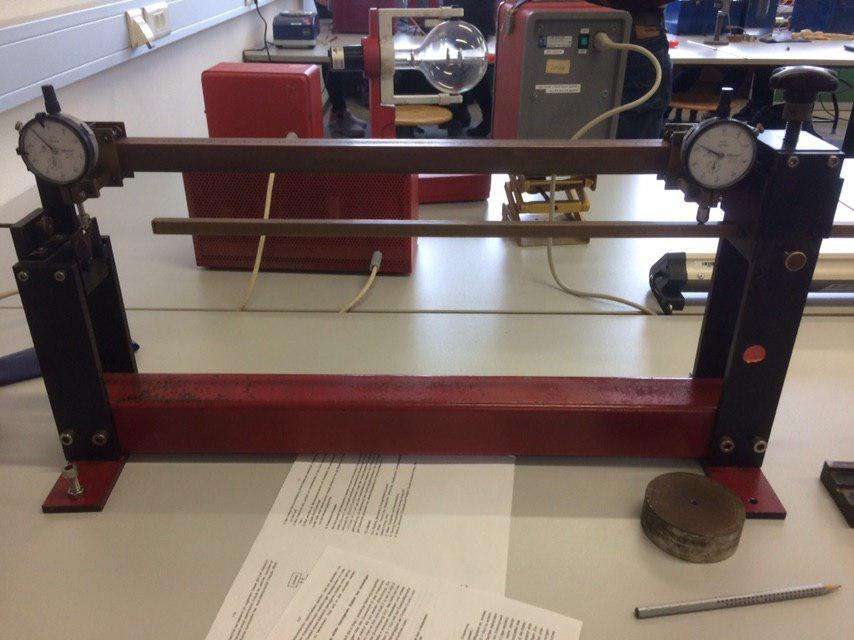
\includegraphics[width=1\linewidth, height=1\linewidth]{Einseitig.jpg}
      \caption{Hier ist der rechteckige Stab einseitig auf der rechten Seite eingespannt. Über ihm sind die auf einer Centimeterskala befestigten Messuhren zu sehen.}
    \end{figure}
    \newpage
    \begin{figure}[h]
      \centering
      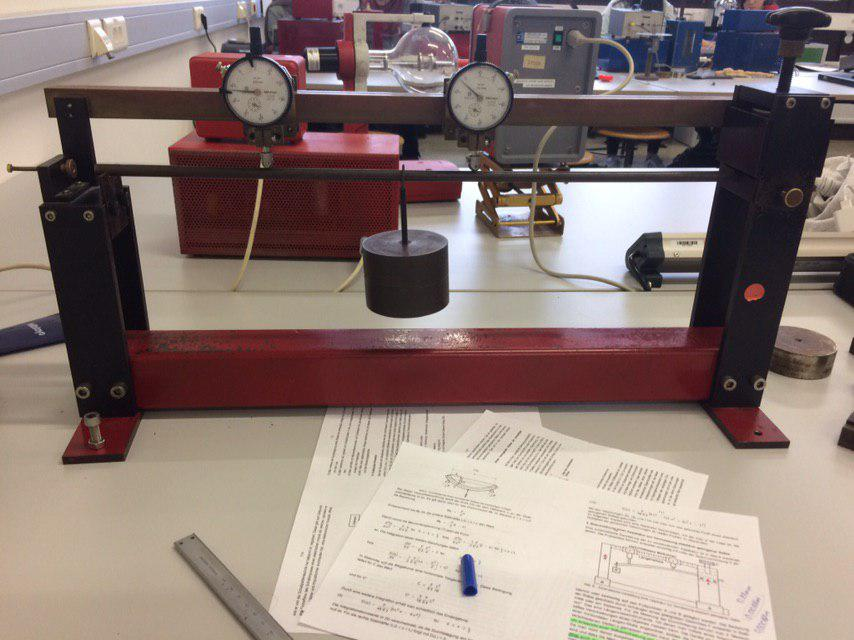
\includegraphics[width=1\linewidth, height=1\linewidth]{Zweiseitig.jpg}
      \caption{Nun ist der runde Stab beidseitig eingespannt. Es ist gut zu erkennen, dass das Gewicht in der Mitte zwischen den zwei Auflagepunkten befestigt ist. }
    \end{figure}
    Zur Messung der Auslenkung werden Messuhren verwendet. Diese bestehen aus einem, an einer Feder befestigten, Messtaster und einer runden Skala. Wenn der 
    Messtaster eingedrückt wird, wird die Distanz auf der Rundskala, die von 0,01 bis 10 Millimeter geht, angezeigt. Mit diesen Messuhren wird vor Beginn der
    Messung der Auslenkung des Stabes über den unausgelenkten Stab gefahren, um die Auslenkung in der Ruhelage zu messen. Dies ist notwendig, da die Stäbe 
    bereits sehr of ausgelenkt worden sind und nie wieder in die ehemalige gerade Form zurückgekehrt sind. Nachdem auf diese Weise, die Ruheauslenkung 
    festgestellt worden ist, wird das Gewicht angehangen und erneut mit den Messuhren über den Stab gefahren. Dabei werden in Abständen von 3 cm die realtiven 
    Auslenkungen gemessen. Im Nachhinein werden die Ruheauslenkungen von den realtiven Auslenkungen abgezogen, um die tatsächliche Auslenkung des Stabes zu
    messen. Da die Messuhr bei zweiseitiger Einspannung in der Mitte blockiert wird, muss in diesem Fall mit zwei verschiedenen Messuhren gemessen werden. Dies
    kann zu unterschieden in den Messergebnissen führen, da bei unserem Experiment besonders eine der Uhren sehr unzuverlässige Werte lieferte.
    \begin{figure}[h]
      \centering
      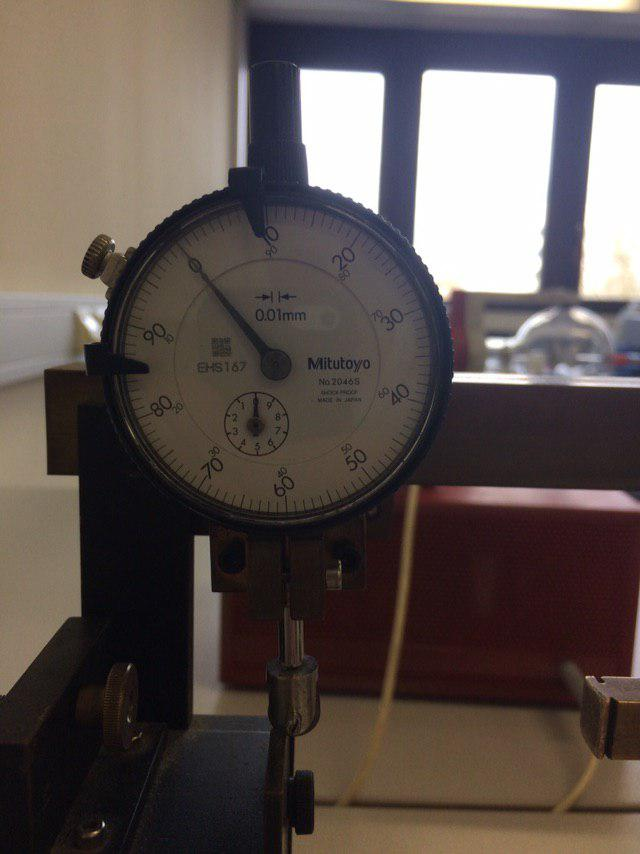
\includegraphics[width=1\linewidth, height=1\linewidth]{Messuhr.jpg}
      \caption{Zu sehen ist eine der mechanischen Messuhren, die zur Bestimmung der Auslenkung genutzt worden ist. Sie ist auf 0,01mm genau und kann Längen bis zu 10mm messen.}
    \end{figure}   

  \end{document}